\chapter{Meiose en genetisch schudden}\label{ch:g12:meiosis-genetic-shuffling}

Twee ouders met elk 46 \omterm{def:g10:universal-dna:information}{chromosomen} krijgen een kind met 46 --- en niet
92. Ergens tussen het lichaam van de ouders en het kind wordt het aantal
gehalveerd, en het wordt zo gehalveerd dat elk kind een hand krijgt
uitgedeeld die geen broer of zus ooit heeft gehad: dezelfde ouders,
veertig jaar kinderen, en geen twee gelijk, behalve eeneiige tweelingen.
Het halveren is een bijzondere deling die \omterm{def:g12:meiosis-genetic-shuffling:meiosis}{meiose} heet; het uitdelen is wat
zij onderweg met de \omterm{def:g10:universal-dna:information}{chromosomen} doet. Dit hoofdstuk volgt één \omterm{def:g10:cells-common-unit:cell}{cel} door de
\omterm{def:g12:meiosis-genetic-shuffling:meiosis}{meiose} heen, telt de combinaties die zij kan voortbrengen, en leest de
uitkomsten van kruisingen die van buitenaf onthullen wat er binnenin
gebeurde.

\section{De set halveren}

\begin{definition}[Diploïde, haploïde, meiose]\label{def:g12:meiosis-genetic-shuffling:meiosis}
Een \omterm{def:g10:cells-common-unit:cell}{cel} met twee kopieën van elk \omterm{def:g11:cell-cycle-mitosis:chromosome}{chromosoom} --- één van elke ouder, en
samen een paar \emph{homologe \omterm{def:g10:universal-dna:information}{chromosomen}} --- is
\emph{diploïde}\index{diploïde}, geschreven als $2n$ ($2n = 46$ bij de
mens). Een \omterm{def:g10:cells-common-unit:cell}{cel} met één kopie van elk is \emph{haploïde}\index{haploïde},
geschreven als $n$. De \emph{meiose}\index{meiose} is de reeks van twee
delingen waarmee één diploïde \omterm{def:g10:cells-common-unit:cell}{cel}, na één enkele verdubbeling van haar
\omterm{def:g10:universal-dna:information}{DNA}, vier haploïde \omterm{def:g10:cells-common-unit:cell}{cellen} voortbrengt --- de gameten, of hun voorlopers.
De \emph{bevruchting} verenigt twee haploïde gameten en herstelt het
diploïde aantal: het afwisselen van meiose en bevruchting is de kringloop
van elke \omterm{def:g10:biodiversity-scales:species}{soort} die zich geslachtelijk voortplant.
\end{definition}

\begin{proposition}[De twee delingen]\label{prop:g12:meiosis-genetic-shuffling:divisions}
Vóór de \omterm{def:g12:meiosis-genetic-shuffling:meiosis}{meiose} wordt het \omterm{def:g10:universal-dna:information}{DNA} verdubbeld: elk \omterm{def:g11:cell-cycle-mitosis:chromosome}{chromosoom} heeft twee
\omterm{def:g11:cell-cycle-mitosis:chromosome}{chromatiden}. Daarna:
\begin{itemize}
  \item \emph{Eerste deling} (\omterm{def:g12:meiosis-genetic-shuffling:meiosis}{meiose} I, \emph{reductiedeling}): de
        homologe \omterm{def:g10:universal-dna:information}{chromosomen} gaan twee aan twee gepaard op de evenaar
        staan; de leden van elk paar worden naar tegenovergestelde polen
        getrokken. Elke dochtercel ontvangt \emph{één \omterm{def:g11:cell-cycle-mitosis:chromosome}{chromosoom} van elk
        paar}, nog altijd uit twee \omterm{def:g11:cell-cycle-mitosis:chromosome}{chromatiden} opgebouwd: $n$
        \omterm{def:g10:universal-dna:information}{chromosomen}, DNA-hoeveelheid $q$ (de hoeveelheid van een
        \omterm{def:g12:meiosis-genetic-shuffling:meiosis}{diploïde} \omterm{def:g10:cells-common-unit:cell}{cel} vóór de verdubbeling).
  \item \emph{Tweede deling} (\omterm{def:g12:meiosis-genetic-shuffling:meiosis}{meiose} II, \emph{gelijkmakende deling}):
        net als bij een \omterm{def:g11:cell-cycle-mitosis:cycle}{mitose} gaan de \omterm{def:g11:cell-cycle-mitosis:chromosome}{chromatiden} van elk \omterm{def:g11:cell-cycle-mitosis:chromosome}{chromosoom}
        uiteen. Elk van de vier \omterm{def:g10:cells-common-unit:cell}{cellen} ontvangt $n$ \omterm{def:g10:universal-dna:information}{chromosomen} met één
        \omterm{def:g11:cell-cycle-mitosis:chromosome}{chromatide}, DNA-hoeveelheid $q/2$.
\end{itemize}
De eerste deling halveert het aantal \omterm{def:g10:universal-dna:information}{chromosomen}; de tweede halveert de
hoeveelheid \omterm{def:g10:universal-dna:information}{DNA} terug tot één \omterm{def:g11:cell-cycle-mitosis:chromosome}{chromatide} per \omterm{def:g11:cell-cycle-mitosis:chromosome}{chromosoom}.
\end{proposition}
\admitted

\begin{omfigure}
\begin{tikzpicture}[font=\small, line cap=round]
  \tikzset{cellb/.style={draw, thick, fill=omDef!5, rounded corners=9pt, minimum width=2.5cm, minimum height=2.5cm},
           ma/.style={line width=3pt, omDef!80}, mb/.style={line width=3pt, omThm!80},
           mA/.style={line width=3pt, omDef!35}, mB/.style={line width=3pt, omThm!35}, cen/.style={fill=black}}
  % panel 1: diploid cell after S: two pairs (long pair blue, short pair red); paternal dark, maternal pale
  \begin{scope}
    \node[cellb] at (0,0) {};
    \draw[ma] (-0.75,0.7) .. controls (-0.62,0.1) .. (-0.75,-0.5); \draw[ma] (-0.49,0.7) .. controls (-0.62,0.1) .. (-0.49,-0.5); \fill[cen] (-0.62,0.1) circle (1.6pt);
    \draw[mA] (-0.2,0.7) .. controls (-0.07,0.1) .. (-0.2,-0.5); \draw[mA] (0.06,0.7) .. controls (-0.07,0.1) .. (0.06,-0.5); \fill[cen] (-0.07,0.1) circle (1.6pt);
    \draw[mb] (0.4,0.45) .. controls (0.53,0.1) .. (0.4,-0.25); \draw[mb] (0.66,0.45) .. controls (0.53,0.1) .. (0.66,-0.25); \fill[cen] (0.53,0.1) circle (1.6pt);
    \draw[mB] (0.9,0.45) .. controls (1.03,0.1) .. (0.9,-0.25); \draw[mB] (1.16,0.45) .. controls (1.03,0.1) .. (1.16,-0.25); \fill[cen] (1.03,0.1) circle (1.6pt);
    \node[anchor=north, align=center, font=\scriptsize, text width=3.05cm] at (0,-1.35) {na de verdubbeling:\\ $2n = 4$, DNA $2q$};
  \end{scope}
  % panel 2: metaphase I: pairs on the equator
  \begin{scope}[xshift=3.2cm]
    \node[cellb] at (0,0) {};
    \draw[dashed, gray] (-1.1,0) -- (1.1,0);
    \draw[ma] (-0.7,0.55) .. controls (-0.57,0.1) .. (-0.7,-0.35); \draw[ma] (-0.44,0.55) .. controls (-0.57,0.1) .. (-0.44,-0.35); \fill[cen] (-0.57,0.15) circle (1.6pt);
    \draw[mA] (-0.7,-0.05) .. controls (-0.57,-0.5) .. (-0.7,-0.95); \draw[mA] (-0.44,-0.05) .. controls (-0.57,-0.5) .. (-0.44,-0.95); \fill[cen] (-0.57,-0.15) circle (1.6pt);
    \draw[mb] (0.45,0.5) .. controls (0.58,0.2) .. (0.45,-0.1); \draw[mb] (0.71,0.5) .. controls (0.58,0.2) .. (0.71,-0.1); \fill[cen] (0.58,0.15) circle (1.6pt);
    \draw[mB] (0.45,0.1) .. controls (0.58,-0.2) .. (0.45,-0.5); \draw[mB] (0.71,0.1) .. controls (0.58,-0.2) .. (0.71,-0.5); \fill[cen] (0.58,-0.15) circle (1.6pt);
    \node[anchor=north, align=center, font=\scriptsize, text width=3.05cm] at (0,-1.35) {meiose I: homologe\\ paren op de evenaar};
  \end{scope}
  % panel 3: two cells after MI, each n=2 with two chromatids
  \begin{scope}[xshift=6.4cm]
    \node[cellb, minimum height=1.15cm] at (0,0.7) {};
    \node[cellb, minimum height=1.15cm] at (0,-0.7) {};
    \draw[ma] (-0.55,1.15) .. controls (-0.42,0.7) .. (-0.55,0.25); \draw[ma] (-0.29,1.15) .. controls (-0.42,0.7) .. (-0.29,0.25); \fill[cen] (-0.42,0.7) circle (1.6pt);
    \draw[mB] (0.35,1.0) .. controls (0.48,0.7) .. (0.35,0.4); \draw[mB] (0.61,1.0) .. controls (0.48,0.7) .. (0.61,0.4); \fill[cen] (0.48,0.7) circle (1.6pt);
    \draw[mA] (-0.55,-0.25) .. controls (-0.42,-0.7) .. (-0.55,-1.15); \draw[mA] (-0.29,-0.25) .. controls (-0.42,-0.7) .. (-0.29,-1.15); \fill[cen] (-0.42,-0.7) circle (1.6pt);
    \draw[mb] (0.35,-0.4) .. controls (0.48,-0.7) .. (0.35,-1.0); \draw[mb] (0.61,-0.4) .. controls (0.48,-0.7) .. (0.61,-1.0); \fill[cen] (0.48,-0.7) circle (1.6pt);
    \node[anchor=north, align=center, font=\scriptsize, text width=3.05cm] at (0,-1.35) {twee cellen: $n = 2$,\\ twee chromatiden, DNA $q$};
  \end{scope}
  % panel 4: four cells after MII, single chromatids
  \begin{scope}[xshift=9.6cm]
    \foreach \y in {1.05,0.35,-0.35,-1.05} \node[cellb, minimum height=0.6cm, minimum width=2.3cm] at (0,\y) {};
    \draw[ma] (-0.5,1.3) -- (-0.5,0.8); \fill[cen] (-0.5,1.05) circle (1.4pt); \draw[mB] (0.4,1.22) -- (0.4,0.88); \fill[cen] (0.4,1.05) circle (1.4pt);
    \draw[ma] (-0.5,0.6) -- (-0.5,0.1); \fill[cen] (-0.5,0.35) circle (1.4pt); \draw[mB] (0.4,0.52) -- (0.4,0.18); \fill[cen] (0.4,0.35) circle (1.4pt);
    \draw[mA] (-0.5,-0.1) -- (-0.5,-0.6); \fill[cen] (-0.5,-0.35) circle (1.4pt); \draw[mb] (0.4,-0.18) -- (0.4,-0.52); \fill[cen] (0.4,-0.35) circle (1.4pt);
    \draw[mA] (-0.5,-0.8) -- (-0.5,-1.3); \fill[cen] (-0.5,-1.05) circle (1.4pt); \draw[mb] (0.4,-0.88) -- (0.4,-1.22); \fill[cen] (0.4,-1.05) circle (1.4pt);
    \node[anchor=north, align=center, font=\scriptsize, text width=3.05cm] at (0,-1.45) {vier gameten: $n = 2$,\\ één chromatide, DNA $q/2$};
  \end{scope}
\end{tikzpicture}

{\small \omterm{def:g12:meiosis-genetic-shuffling:meiosis}{Meiose} in een \omterm{def:g10:cells-common-unit:cell}{cel} met twee paren \omterm{def:g10:universal-dna:information}{chromosomen} ($2n = 4$); donkere
en bleke tinten geven de twee leden van elk paar aan, van de twee ouders.
De eerste deling scheidt de homologen, de tweede de \omterm{def:g11:cell-cycle-mitosis:chromosome}{chromatiden}. Hier ging
het donkere lange \omterm{def:g11:cell-cycle-mitosis:chromosome}{chromosoom} met het bleke korte mee: een van de twee
mogelijke verdelingen.}
\end{omfigure}

\begin{omfigure}
\begin{tikzpicture}
\begin{axis}[
  width=0.88\linewidth, height=5.2cm,
  axis x line=bottom, axis y line=left,
  xmin=0, xmax=10, ymin=0, ymax=2.7,
  xlabel={tijd}, ylabel={DNA per cel},
  xlabel style={font=\small, at={(axis description cs:0.5,-0.1)}, anchor=north},
  ylabel style={font=\small},
  tick label style={font=\small}, xtick=\empty,
  ytick={0.5,1,2}, yticklabels={$q/2$, $q$, $2q$},
  clip=false,
]
\addplot[thick, omDef] coordinates {(0,1) (2,1) (4,2) (5.9,2) (6,1) (7.9,1) (8,0.5) (10,0.5)};
\draw[dashed, gray] (axis cs:2,0) -- (axis cs:2,2.2); \draw[dashed, gray] (axis cs:4,0) -- (axis cs:4,2.2);
\draw[dashed, gray] (axis cs:6,0) -- (axis cs:6,2.2); \draw[dashed, gray] (axis cs:8,0) -- (axis cs:8,2.2);
\node[font=\small, anchor=south] at (axis cs:1,2.25) {$2n$, $q$};
\node[font=\small, anchor=south] at (axis cs:3,2.25) {S-fase};
\node[font=\small, anchor=south] at (axis cs:5,2.25) {$2n$, $2q$};
\node[font=\small, anchor=south, omThm] at (axis cs:6,2.45) {meiose I};
\node[font=\small, anchor=south] at (axis cs:7,2.25) {$n$, $q$};
\node[font=\small, anchor=south, omThm] at (axis cs:8,2.45) {meiose II};
\node[font=\small, anchor=south] at (axis cs:9,2.25) {$n$, $q/2$};
\end{axis}
\end{tikzpicture}

{\small \omterm{def:g10:universal-dna:information}{DNA} per \omterm{def:g10:cells-common-unit:cell}{cel} door de \omterm{def:g12:meiosis-genetic-shuffling:meiosis}{meiose} heen. Eén verdubbeling, en daarna twee
delingen zonder verdubbeling ertussen: de gameten bevatten een kwart van
het \omterm{def:g10:universal-dna:information}{DNA} dat de moedercel na S bevatte, en de helft van wat een \omterm{def:g12:meiosis-genetic-shuffling:meiosis}{diploïde}
\omterm{def:g10:cells-common-unit:cell}{cel} in rust bevat.}
\end{omfigure}

\begin{example}[Menselijke getallen]\label{ex:g12:meiosis-genetic-shuffling:numbers}
Een kiemcel van de teelbal, $2n = 46$, verdubbelt tot 46 \omterm{def:g10:universal-dna:information}{chromosomen} met
twee \omterm{def:g11:cell-cycle-mitosis:chromosome}{chromatiden} ($2q$); na \omterm{def:g12:meiosis-genetic-shuffling:meiosis}{meiose} I zijn er twee \omterm{def:g10:cells-common-unit:cell}{cellen} met 23
\omterm{def:g10:universal-dna:information}{chromosomen} van twee \omterm{def:g11:cell-cycle-mitosis:chromosome}{chromatiden} ($q$); na \omterm{def:g12:meiosis-genetic-shuffling:meiosis}{meiose} II vier zaadcellen met
23 \omterm{def:g10:universal-dna:information}{chromosomen} van één \omterm{def:g11:cell-cycle-mitosis:chromosome}{chromatide} ($q/2$). Bij de bevruchting geldt $23 + 23 =
46$ en $q/2 + q/2 = q$: de bevruchte eicel is terug bij een \omterm{def:g12:meiosis-genetic-shuffling:meiosis}{diploïde} \omterm{def:g10:cells-common-unit:cell}{cel}
in rust. In de eierstok brengen dezelfde delingen één grote
eicel voort en drie piepkleine \omterm{def:g10:cells-common-unit:cell}{cellen} die worden weggeworpen; de
rekensom is dezelfde.
\end{example}

\section{Het schudden}

\begin{proposition}[Onafhankelijke verdeling]\label{prop:g12:meiosis-genetic-shuffling:assortment}
In de metafase I gaat elk paar homologen onafhankelijk van de andere
paren op de evenaar staan: welk lid van een paar naar welke pool gaat,
wordt paar voor paar door het toeval bepaald. Een \omterm{def:g10:cells-common-unit:cell}{cel} met $n$ paren kan
dus $2^n$ verschillende combinaties van vaderlijke en moederlijke
\omterm{def:g10:universal-dna:information}{chromosomen} in haar gameten voortbrengen --- $2^{23} \approx \num{8.4e6}$
bij de mens. De bevruchting, die twee van zulke gameten willekeurig
verenigt, levert $2^{23}
\times 2^{23} \approx \num{7e13}$ chromosoomcombinaties op voor de
kinderen van één paar, nog vóór enige andere bron van verscheidenheid is
meegeteld.
\end{proposition}
\admitted

\begin{proposition}[Crossing-over]\label{prop:g12:meiosis-genetic-shuffling:crossingover}
Terwijl de homologen gepaard zijn, vroeg in \omterm{def:g12:meiosis-genetic-shuffling:meiosis}{meiose} I, breken twee
\omterm{def:g11:cell-cycle-mitosis:chromosome}{chromatiden} die geen zusters van elkaar zijn op hetzelfde punt en
verbinden zij zich kruiselings opnieuw: een
\emph{crossing-over}\index{crossing-over}. Elke \omterm{def:g11:cell-cycle-mitosis:chromosome}{chromatide} draagt voorbij
het uitwisselingspunt nu de \omterm{def:g10:universal-dna:gene}{allelen} van de andere \omterm{def:g10:common-ancestry:homology}{homoloog}. De
\omterm{def:g10:universal-dna:information}{chromosomen} die de gameten bereiken zijn dus niet de \omterm{def:g10:universal-dna:information}{chromosomen} van de
ouders maar \emph{gerecombineerde} \omterm{def:g10:universal-dna:information}{chromosomen}, die over hun lengte de
\omterm{def:g10:universal-dna:gene}{allelen} van de twee grootouders mengen. Bij elke \omterm{def:g12:meiosis-genetic-shuffling:meiosis}{meiose} vinden op elk
paar één tot drie uitwisselingen plaats, op wisselende plaatsen: het
aantal mogelijke gameten is in de praktijk onbeperkt.
\end{proposition}
\begin{proof}[Bewijsmateriaal]
Onder de microscoop tonen gepaarde homologen in \omterm{def:g12:meiosis-genetic-shuffling:meiosis}{meiose} I gekruiste
punten, \emph{chiasmata}, waar twee \omterm{def:g11:cell-cycle-mitosis:chromosome}{chromatiden} zichtbaar van partner
wisselen. Kruisingen waarbij twee \omterm{def:g10:universal-dna:gene}{genen} op hetzelfde \omterm{def:g11:cell-cycle-mitosis:chromosome}{chromosoom} liggen,
geven onder de nakomelingen een minderheid met nieuwe combinaties van de
\omterm{def:g10:universal-dna:gene}{allelen} van de twee \omterm{def:g10:universal-dna:gene}{genen} --- combinaties die geen van beide ouders had ---
in een verhouding die van de afstand tussen de \omterm{def:g10:universal-dna:gene}{genen} afhangt; \omterm{def:g10:universal-dna:gene}{genen} die
ver uit elkaar op een \omterm{def:g11:cell-cycle-mitosis:chromosome}{chromosoom} liggen, recombineren even vaak als \omterm{def:g10:universal-dna:gene}{genen}
op verschillende \omterm{def:g10:universal-dna:information}{chromosomen}. Moleculaire merkers die door families heen
worden gevolgd, laten de stukken van elk \omterm{def:g11:cell-cycle-mitosis:chromosome}{chromosoom} per generatie op één
of twee punten van grootouderlijke herkomst wisselen.
\end{proof}

\begin{omfigure}
\begin{tikzpicture}[font=\small, line cap=round, >=Stealth]
  \tikzset{p/.style={line width=4pt, omDef!80}, m/.style={line width=4pt, omThm!70}}
  % before: two homologues, each two chromatids; alleles A/a, B/b
  \draw[p] (0,0) -- (0,3); \draw[p] (0.35,0) -- (0.35,3);
  \draw[m] (0.9,0) -- (0.9,3); \draw[m] (1.25,0) -- (1.25,3);
  \foreach \x in {0,0.35} { \node[font=\scriptsize, anchor=east, xshift=-1pt] at (\x,2.6) {}; }
  \node[font=\scriptsize, omDef!80!black, anchor=east] at (-0.15,2.6) {$A$};
  \node[font=\scriptsize, omDef!80!black, anchor=east] at (-0.15,0.5) {$B$};
  \node[font=\scriptsize, omThm!80!black, anchor=west] at (1.4,2.6) {$a$};
  \node[font=\scriptsize, omThm!80!black, anchor=west] at (1.4,0.5) {$b$};
  \node[anchor=north, align=center] at (0.62,-0.2) {gepaarde homologen\\ (elk twee chromatiden)};
  \draw[->, thick] (2.4,1.5) -- (3.4,1.5);
  % during: chiasma between the two inner chromatids at y=1.5
  \begin{scope}[xshift=4.2cm]
    \draw[p] (0,0) -- (0,3);
    \draw[p] (0.35,3) -- (0.35,1.6) -- (0.9,1.4) -- (0.9,0);
    \draw[m] (0.9,3) -- (0.9,1.6) -- (0.35,1.4) -- (0.35,0);
    \draw[m] (1.25,0) -- (1.25,3);
    \node[anchor=north, align=center] at (0.62,-0.2) {chiasma: twee chromatiden\\ breken en verbinden kruiselings};
  \end{scope}
  \draw[->, thick] (6.6,1.5) -- (7.6,1.5);
  % after: four chromatids separated
  \begin{scope}[xshift=8.4cm]
    \draw[p] (0,0) -- (0,3);
    \draw[p] (0.5,3) -- (0.5,1.5); \draw[m] (0.5,1.5) -- (0.5,0);
    \draw[m] (1.0,3) -- (1.0,1.5); \draw[p] (1.0,1.5) -- (1.0,0);
    \draw[m] (1.5,0) -- (1.5,3);
    \node[font=\scriptsize, anchor=south] at (0,3.05) {$AB$};
    \node[font=\scriptsize, anchor=south] at (0.5,3.05) {$Ab$};
    \node[font=\scriptsize, anchor=south] at (1.0,3.05) {$aB$};
    \node[font=\scriptsize, anchor=south] at (1.5,3.05) {$ab$};
    \node[anchor=north, align=center] at (0.75,-0.2) {vier gameten: twee ouderlijk,\\ twee gerecombineerd};
  \end{scope}
\end{tikzpicture}

{\small \omterm{prop:g12:meiosis-genetic-shuffling:crossingover}{Crossing-over} tussen twee \omterm{def:g10:universal-dna:gene}{genen} $A$ en $B$ op hetzelfde
\omterm{def:g11:cell-cycle-mitosis:chromosome}{chromosoom}. Twee van de vier \omterm{def:g11:cell-cycle-mitosis:chromosome}{chromatiden} wisselen hun uiteinden uit; van
de vier gameten dragen er twee de ouderlijke combinaties ($AB$, $ab$) en
twee nieuwe ($Ab$, $aB$).}
\end{omfigure}

\begin{omfigure}
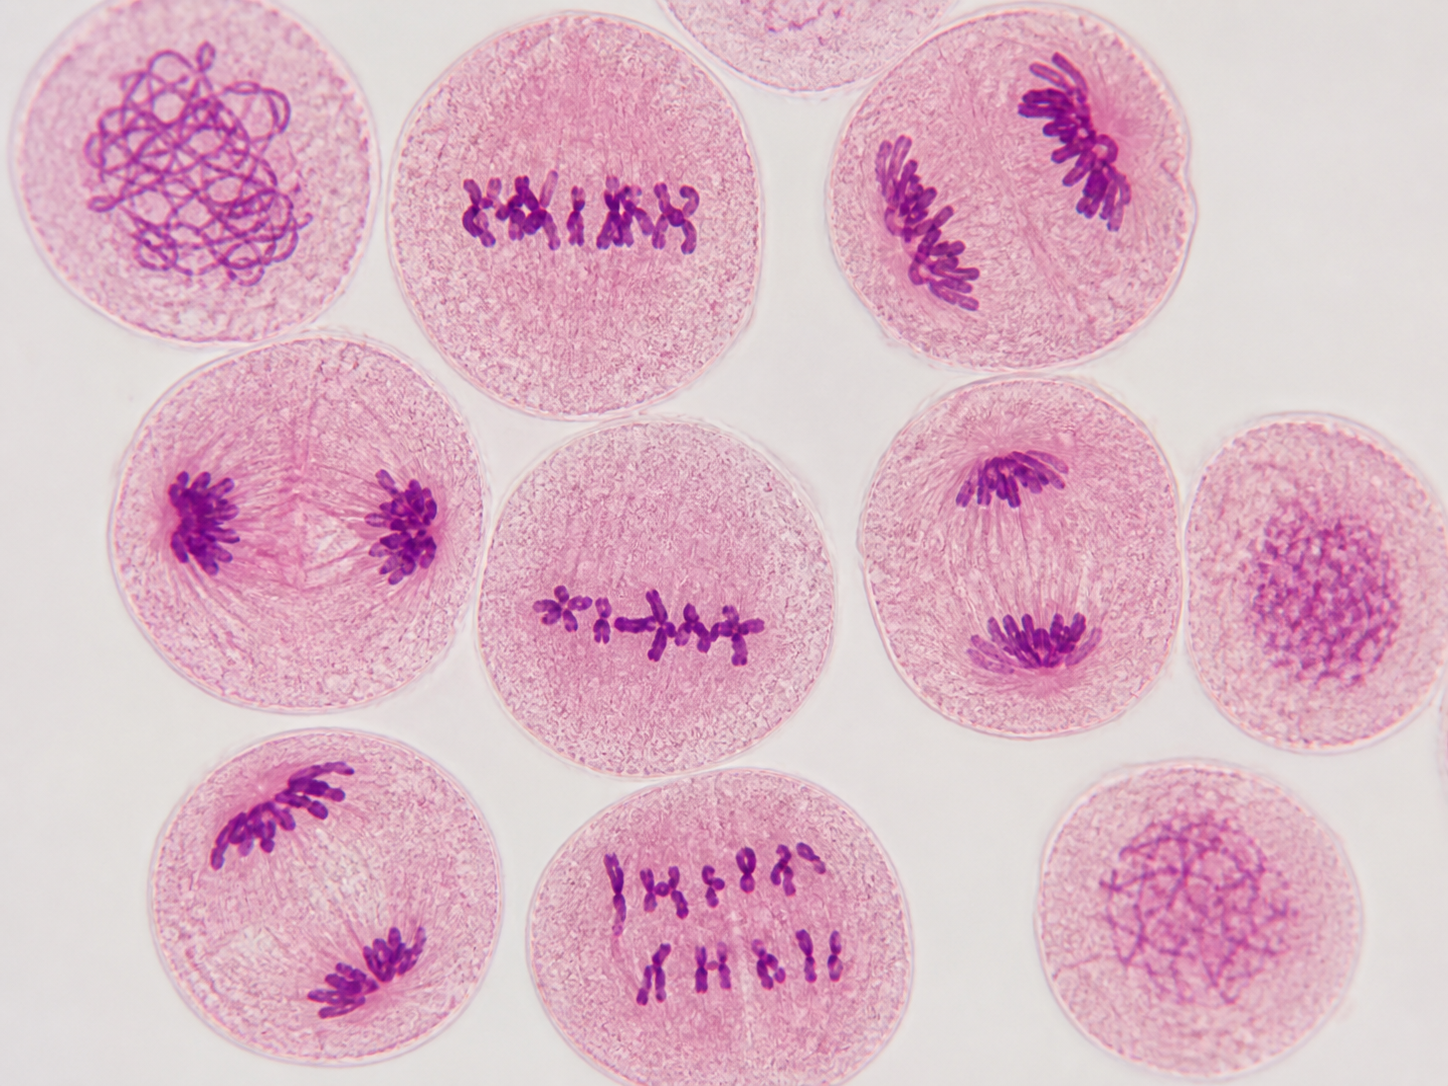
\includegraphics[width=0.56\linewidth]{images/book2/ai/g12-meiosis-lily-anther.png}

{\small \omterm{def:g10:cells-common-unit:cell}{Cellen} uit een lelieheelmknop in \omterm{def:g12:meiosis-genetic-shuffling:meiosis}{meiose}, gekleurd: bij sommige
staan de gepaarde homologen midden in de \omterm{def:g10:cells-common-unit:cell}{cel} op een rij; bij andere zijn
zij naar de twee polen getrokken. De stadia van het schema, gezien in het
weefsel dat stuifmeel maakt.}
\end{omfigure}

\begin{example}[Drie bronnen van verscheidenheid, op volgorde]\label{ex:g12:meiosis-genetic-shuffling:sources}
Een kind van twee ouders is op drie manieren nieuw: de \omterm{prop:g12:meiosis-genetic-shuffling:crossingover}{crossing-over}
bouwde elk \omterm{def:g11:cell-cycle-mitosis:chromosome}{chromosoom} van elke gameet opnieuw op uit de twee
grootouderlijke kopieën; de onafhankelijke verdeling deelde van elk paar
één gerecombineerd \omterm{def:g11:cell-cycle-mitosis:chromosome}{chromosoom} in de gameet uit, uit $2^{23}$ mogelijke
verdelingen; de bevruchting koppelde zo'n gameet aan een gameet die uit
de $2^{23}$ van de andere ouder was getrokken. De \omterm{def:g11:mutations:mutation}{mutatie}, die de \omterm{def:g10:universal-dna:gene}{allelen}
schiep die worden geschud, werkt op een veel tragere tijdschaal: het
schudden is wat elke generatie nieuw maakt uit hetzelfde kaartspel.
\end{example}

\section{Het schudden aflezen in een kruising}

\begin{omfigure}
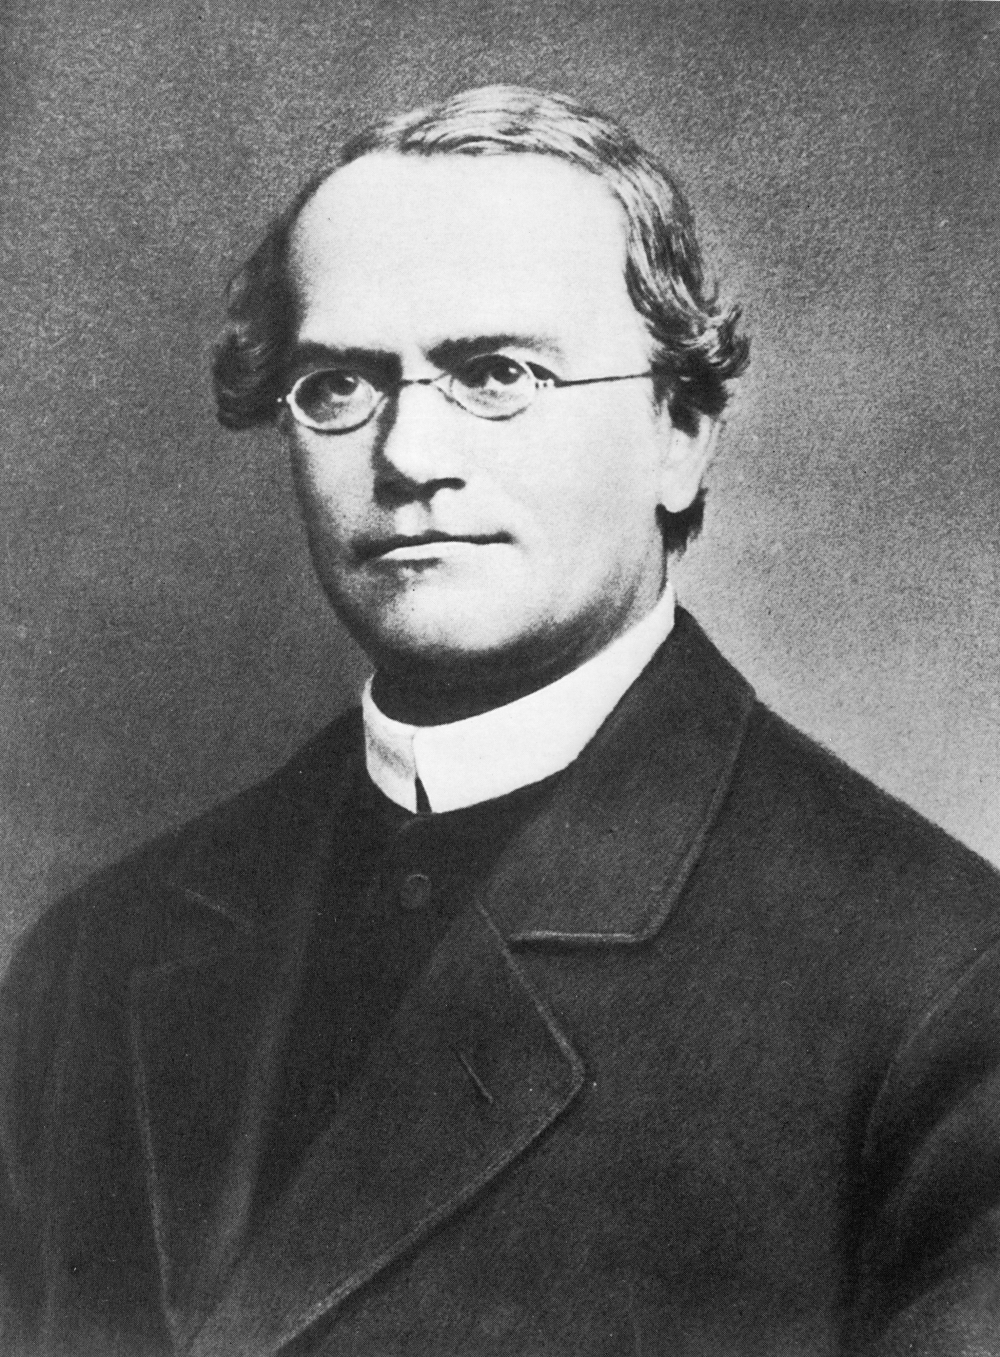
\includegraphics[width=0.3\linewidth]{images/book2/mendel.jpg}

{\small Gregor Mendel, die in de jaren zestig van de negentiende eeuw in een kloostertuin de nakomelingen van erwtenkruisingen telde en de verhoudingen vond --- 3:1 voor één kenmerk, 9:3:3:1 voor twee --- die de \omterm{def:g12:meiosis-genetic-shuffling:meiosis}{meiose}, buiten zijn weten om, voortbrengt. Foto, publiek domein.}
\end{omfigure}

\begin{method}[De testkruising]\label{met:g12:meiosis-genetic-shuffling:testcross}
Om te zien welke gameten een individu maakt, kruis je het met een partner
die alleen recessieve \omterm{def:g10:universal-dna:gene}{allelen} draagt (een \emph{testkruising}): elke
nakomeling toont dan precies de \omterm{def:g10:universal-dna:gene}{allelen} die de gameet van de geteste
ouder droeg. Voor twee \omterm{def:g10:universal-dna:gene}{genen}, met de geteste ouder $AaBb$ en de partner
$aabb$:
\begin{enumerate}
  \item Tel de vier typen nakomelingen: $AB$, $Ab$, $aB$, $ab$ (die
        elk ook $ab$ van de partner dragen).
  \item Komen de vier even vaak voor ($1:1:1:1$), dan liggen de \omterm{def:g10:universal-dna:gene}{genen} op
        verschillende \omterm{def:g10:universal-dna:information}{chromosomen} en verdelen zij zich onafhankelijk.
  \item Zijn twee typen (de ouderlijke combinaties) veel talrijker dan
        de andere twee (de recombinanten), dan liggen de \omterm{def:g10:universal-dna:gene}{genen} op
        hetzelfde \omterm{def:g11:cell-cycle-mitosis:chromosome}{chromosoom}; de recombinanten komen van \omterm{prop:g12:meiosis-genetic-shuffling:crossingover}{crossing-over},
        en hun aandeel meet de afstand tussen de \omterm{def:g10:universal-dna:gene}{genen}.
  \item Recombinanten zijn altijd de minderheid en komen altijd in twee
        even grote klassen; de ouderlijke eveneens.
\end{enumerate}
\end{method}

\begin{example}[Twee kruisingen bij de fruitvlieg]\label{ex:g12:meiosis-genetic-shuffling:fly}
Vlieg A, heterozygoot voor lichaamskleur en vleugelvorm, testgekruist:
254 grijs-normaal, 248 zwart-rudimentair, 251 grijs-rudimentair, 247
zwart-normaal --- vier even grote klassen, de \omterm{def:g10:universal-dna:gene}{genen} liggen op
verschillende \omterm{def:g10:universal-dna:information}{chromosomen}. Vlieg B, heterozygoot voor lichaamskleur en
oogkleur: 412 grijs-rood, 405 zwart-purper, 44 grijs-purper, 39 zwart-rood
--- twee ouderlijke klassen van elk ongeveer 45\% en twee recombinante
klassen van ongeveer 5\%: de \omterm{def:g10:universal-dna:gene}{genen} liggen op hetzelfde \omterm{def:g11:cell-cycle-mitosis:chromosome}{chromosoom}, dicht
bij elkaar, en worden in 9\% van de \omterm{def:g12:meiosis-genetic-shuffling:meiosis}{meiosen} door een \omterm{prop:g12:meiosis-genetic-shuffling:crossingover}{crossing-over}
gescheiden.
\end{example}

\begin{omfigure}
\begin{tikzpicture}[font=\small]
  \draw[thick] (0,0) grid[step=1.4] (5.6,1.4);
  \node[fill=omDef!15, minimum width=1.3cm, minimum height=1.3cm, align=center] at (0.7,0.7) {$AB$\\ 254};
  \node[fill=omDef!15, minimum width=1.3cm, minimum height=1.3cm, align=center] at (2.1,0.7) {$Ab$\\ 251};
  \node[fill=omDef!15, minimum width=1.3cm, minimum height=1.3cm, align=center] at (3.5,0.7) {$aB$\\ 247};
  \node[fill=omDef!15, minimum width=1.3cm, minimum height=1.3cm, align=center] at (4.9,0.7) {$ab$\\ 248};
  \node[anchor=south] at (2.8,1.5) {vlieg A: onafhankelijke genen, $1:1:1:1$};
  \begin{scope}[xshift=7.4cm]
    \draw[thick] (0,0) grid[step=1.4] (5.6,1.4);
    \node[fill=omProp!25, minimum width=1.3cm, minimum height=1.3cm, align=center] at (0.7,0.7) {$AB$\\ 412};
    \node[fill=omThm!20, minimum width=1.3cm, minimum height=1.3cm, align=center] at (2.1,0.7) {$Ab$\\ 44};
    \node[fill=omThm!20, minimum width=1.3cm, minimum height=1.3cm, align=center] at (3.5,0.7) {$aB$\\ 39};
    \node[fill=omProp!25, minimum width=1.3cm, minimum height=1.3cm, align=center] at (4.9,0.7) {$ab$\\ 405};
    \node[anchor=south] at (2.8,1.5) {vlieg B: gekoppelde genen, ouderlijk $\gg$ recombinant};
  \end{scope}
\end{tikzpicture}

{\small De gameten van twee heterozygote vliegen, afgelezen uit
testkruisingen. Even grote klassen betekenen onafhankelijke verdeling;
twee grote en twee kleine klassen betekenen dat de \omterm{def:g10:universal-dna:gene}{genen} gekoppeld zijn,
waarbij de kleine klassen door \omterm{prop:g12:meiosis-genetic-shuffling:crossingover}{crossing-over} ontstaan.}
\end{omfigure}

\section{Wanneer het schudden misgaat}

\begin{proposition}[Fouten in de meiose]\label{prop:g12:meiosis-genetic-shuffling:errors}
Nu en dan gaat een paar homologen in \omterm{def:g12:meiosis-genetic-shuffling:meiosis}{meiose} I niet uiteen, of gaan twee
\omterm{def:g11:cell-cycle-mitosis:chromosome}{chromatiden} dat niet in \omterm{def:g12:meiosis-genetic-shuffling:meiosis}{meiose} II: de ene gameet krijgt twee kopieën van
een \omterm{def:g11:cell-cycle-mitosis:chromosome}{chromosoom} en de andere geen. Bevrucht geven zij een bevruchte eicel
met drie kopieën (\emph{trisomie}) of met één (\emph{monosomie}). De
meeste van zulke eicellen komen niet tot ontwikkeling; die het wel doen,
dragen een aantal kenmerkende verschijnselen. Trisomie 21 (ongeveer één
geboorte op 700) veroorzaakt een verstandelijke beperking en
hartafwijkingen en is de gewoonste; haar frequentie stijgt steil met de
leeftijd van de moeder. Een ongelijke \omterm{prop:g12:meiosis-genetic-shuffling:crossingover}{crossing-over} --- \omterm{def:g11:cell-cycle-mitosis:chromosome}{chromatiden} die
ongelijke stukken uitwisselen --- levert een \omterm{def:g11:cell-cycle-mitosis:chromosome}{chromosoom} met een verdubbeld
\omterm{def:g10:universal-dna:gene}{gen} en een \omterm{def:g11:cell-cycle-mitosis:chromosome}{chromosoom} met een deletie op: het mechanisme waarmee de
opsinegenen uit \cref{ch:g11:the-eye} zijn vermenigvuldigd, en waarmee
nieuwe \omterm{def:g10:universal-dna:gene}{genen} ontstaan (\cref{ch:g12:diversification-of-life}).
\end{proposition}
\admitted

\begin{omfigure}
\begin{tikzpicture}
\begin{axis}[
  width=0.84\linewidth, height=5.4cm,
  axis x line=bottom, axis y line=left,
  xmin=18, xmax=47, ymin=0, ymax=40,
  xlabel={leeftijd van de moeder (jaar)}, ylabel={trisomie 21 per 1000 geboorten},
  xlabel style={font=\small, at={(axis description cs:0.5,-0.12)}, anchor=north},
  ylabel style={font=\small},
  tick label style={font=\small}, xtick={20,25,30,35,40,45}, ytick={0,10,20,30,40},
]
\addplot[thick, omThm, mark=*, mark size=1.5pt] coordinates
  {(20,0.7) (25,0.8) (30,1.1) (33,1.8) (35,2.9) (37,4.5) (39,7.5) (41,12) (43,20) (45,33)};
\end{axis}
\end{tikzpicture}

{\small De frequentie van trisomie 21 bij de geboorte tegen de leeftijd
van de moeder. De eicellen worden vóór de geboorte van een vrouw gevormd
en blijven tientallen jaren in \omterm{def:g12:meiosis-genetic-shuffling:meiosis}{meiose} I stilstaan; hoe langer die stilstand
duurt, des te waarschijnlijker het is dat de homologen niet uiteengaan.}
\end{omfigure}

\begin{example}[Geslachtschromosomen verkeerd geteld]\label{ex:g12:meiosis-genetic-shuffling:sexchrom}
Een gameet zonder geslachtschromosoom die door een gameet met een X wordt
bevrucht, geeft een XO-eicel: een meisje van geringe lengte bij wie de
eierstokken zich niet ontwikkelen. Een eicel met XX die door een zaadcel
met een Y wordt bevrucht, geeft XXY: een jongen bij wie de teelballen
klein blijven en geen zaadcellen maken. In beide gevallen beslist \omterm{prop:g11:becoming-male-female:sry}{SRY} over
de geslachtsklier, net als in \cref{ch:g11:becoming-male-female}; het
aantal \omterm{def:g10:universal-dna:information}{X-chromosomen} beslist over veel van de rest, en daarom zijn dit de
mildste van de chromosoomfouten.
\end{example}

\begin{remark}[Waarom geslachtelijke voortplanting]\label{rem:g12:meiosis-genetic-shuffling:whysex}
Een bacterie kopieert zichzelf; een roos kan uit een stek groeien.
Geslachtelijke voortplanting is duurder --- twee ouders, een \omterm{def:g12:meiosis-genetic-shuffling:meiosis}{meiose}, het
zoeken van een partner --- en haar product is een reeks nakomelingen die
elk van hun ouders en van elkaar verschillen. Juist dat verschil is het
punt: in een omgeving die verandert, en tegenover parasieten die
evolueren, bevat een populatie van verschillende individuen eerder enkele
die het overleven dan een populatie van kopieën. Het schudden van dit
hoofdstuk is de grondstof die de selectie van de volgende twee
hoofdstukken zal sorteren.
\end{remark}

\section{Oefeningen}

\begin{exercise}[$\star$]\label{exo:g12:meiosis-genetic-shuffling:1}
Definieer \omterm{def:g12:meiosis-genetic-shuffling:meiosis}{diploïde} en \omterm{def:g12:meiosis-genetic-shuffling:meiosis}{haploïde}, en zeg wat de \omterm{def:g12:meiosis-genetic-shuffling:meiosis}{meiose} doet met het aantal
\omterm{def:g10:universal-dna:information}{chromosomen} en met de hoeveelheid \omterm{def:g10:universal-dna:information}{DNA}.
\end{exercise}

\begin{exercise}[$\star$]\label{exo:g12:meiosis-genetic-shuffling:2}
Wat gaat er uiteen in \omterm{def:g12:meiosis-genetic-shuffling:meiosis}{meiose} I? En in \omterm{def:g12:meiosis-genetic-shuffling:meiosis}{meiose} II? Welke deling is de
reductiedeling?
\end{exercise}

\begin{exercise}[$\star$]\label{exo:g12:meiosis-genetic-shuffling:3}
Een \omterm{def:g10:cells-common-unit:cell}{cel} heeft $2n = 8$ en \omterm{def:g10:universal-dna:information}{DNA} $2q$ aan het begin van de \omterm{def:g12:meiosis-genetic-shuffling:meiosis}{meiose}. Geef het
aantal \omterm{def:g10:universal-dna:information}{chromosomen} en de hoeveelheid \omterm{def:g10:universal-dna:information}{DNA} van de \omterm{def:g10:cells-common-unit:cell}{cellen} na \omterm{def:g12:meiosis-genetic-shuffling:meiosis}{meiose} I en na
\omterm{def:g12:meiosis-genetic-shuffling:meiosis}{meiose} II.
\end{exercise}

\begin{exercise}[$\star$]\label{exo:g12:meiosis-genetic-shuffling:4}
Hoeveel chromosoomcombinaties kunnen de gameten van een \omterm{def:g10:biodiversity-scales:species}{soort} met $2n = 8$
alleen al door de onafhankelijke verdeling vertonen?
\end{exercise}

\begin{exercise}[$\star$]\label{exo:g12:meiosis-genetic-shuffling:5}
Wat is een testkruising, en wat onthult het aandeel recombinante
nakomelingen?
\end{exercise}

\begin{exercise}[$\star\star$]\label{exo:g12:meiosis-genetic-shuffling:6}
Lees uit de DNA-figuur het \omterm{def:g10:universal-dna:information}{DNA} per \omterm{def:g10:cells-common-unit:cell}{cel} af van een \omterm{def:g10:cells-common-unit:cell}{cel} in \omterm{def:g12:meiosis-genetic-shuffling:meiosis}{meiose} I, van een
\omterm{def:g10:cells-common-unit:cell}{cel} tussen de twee delingen, en van een gameet. Leg uit waarom er tussen
de delingen geen S-fase ligt.
\end{exercise}

\begin{exercise}[$\star\star$]\label{exo:g12:meiosis-genetic-shuffling:7}
Een testkruising geeft 300 $AB$, 298 $ab$, 302 $Ab$, 300 $aB$. Zijn de
\omterm{def:g10:universal-dna:gene}{genen} gekoppeld? Wat zijn de gameten van de ouder?
\end{exercise}

\begin{exercise}[$\star\star$]\label{exo:g12:meiosis-genetic-shuffling:8}
Een testkruising geeft 460 $AB$, 455 $ab$, 42 $Ab$, 43 $aB$. Zijn de \omterm{def:g10:universal-dna:gene}{genen}
gekoppeld? Welke klassen zijn recombinant, en welk deel vormen zij?
\end{exercise}

\begin{exercise}[$\star\star$]\label{exo:g12:meiosis-genetic-shuffling:9}
Welke twee gameten zou je in de figuur van de \omterm{prop:g12:meiosis-genetic-shuffling:crossingover}{crossing-over} krijgen als de
uitwisseling \emph{boven} beide \omterm{def:g10:universal-dna:gene}{genen} had plaatsgevonden? Leg dat uit.
\end{exercise}

\begin{exercise}[$\star\star$]\label{exo:g12:meiosis-genetic-shuffling:10}
Lees in de trisomiefiguur de frequentie op 25, 35 en 42 jaar af, en
bereken de factor tussen 25 en 42.
\end{exercise}

\begin{exercise}[$\star\star$]\label{exo:g12:meiosis-genetic-shuffling:11}
Leg uit hoe een non-disjunctie in \omterm{def:g12:meiosis-genetic-shuffling:meiosis}{meiose} I verschilt van een in \omterm{def:g12:meiosis-genetic-shuffling:meiosis}{meiose} II
wat betreft de gameten die zij oplevert (kijk naar alle vier de \omterm{def:g10:cells-common-unit:cell}{cellen}).
\end{exercise}

\begin{exercise}[$\star\star\star$]\label{exo:g12:meiosis-genetic-shuffling:12}
Twee \omterm{def:g10:universal-dna:gene}{genen} op hetzelfde \omterm{def:g11:cell-cycle-mitosis:chromosome}{chromosoom} recombineren in 2\% van de \omterm{def:g12:meiosis-genetic-shuffling:meiosis}{meiosen};
twee andere op hetzelfde \omterm{def:g11:cell-cycle-mitosis:chromosome}{chromosoom} in 48\%. Leg uit wat elk getal over
hun onderlinge afstand zegt, en waarom het tweede paar zich vrijwel als
onafhankelijke \omterm{def:g10:universal-dna:gene}{genen} gedraagt.
\end{exercise}

\begin{exercise}[$\star\star\star$]\label{exo:g12:meiosis-genetic-shuffling:13}
Een plant heeft $2n = 4$, waarbij het ene paar $A/a$ draagt en het andere
$B/b$. Noem alle gameten van een $AaBb$-plant met hun frequenties, zonder
\omterm{prop:g12:meiosis-genetic-shuffling:crossingover}{crossing-over}; zeg daarna wat \omterm{prop:g12:meiosis-genetic-shuffling:crossingover}{crossing-over} zou veranderen.
\end{exercise}

\begin{exercise}[$\star\star\star$]\label{exo:g12:meiosis-genetic-shuffling:14}
Eeneiige tweelingen delen al hun \omterm{def:g10:universal-dna:gene}{allelen}; gewone broers en zussen
gemiddeld de helft. Verklaar die "helft" met \omterm{def:g12:meiosis-genetic-shuffling:meiosis}{meiose} en bevruchting, en leg
uit waarom het een gemiddelde is.
\end{exercise}

\begin{exercise}[$\star\star\star$]\label{exo:g12:meiosis-genetic-shuffling:15}
Sommige planten planten zich voort met zaden die zonder \omterm{def:g12:meiosis-genetic-shuffling:meiosis}{meiose} of
bevruchting worden gevormd. Leg uit wat hun nakomelingen genetisch zijn,
wat zo'n plant wint, en wat zij op de lange duur verliest.
\end{exercise}

\section{Probleem: De vliegen van de geneticus}

\begin{problem}[{Weekendprobleem --- twee genen gevolgd door een meiose
en een testkruising: de gameten geteld, de koppeling vastgesteld, de
recombinatie gemeten, en het aantal handen dat een paar kan uitdelen}]
\label{pb:g12:meiosis-genetic-shuffling:1}
Bij de fruitvlieg is het \omterm{def:g10:universal-dna:gene}{allel} $b$ (zwart lichaam) \omterm{def:g11:genes-and-disease:genetic}{recessief} ten opzichte
van $b^+$ (grijs), en $vg$ (rudimentaire vleugels) \omterm{def:g11:genes-and-disease:genetic}{recessief} ten opzichte
van $vg^+$ (normaal). Een grijs vrouwtje met normale vleugels, van wie de
ouders zuiver grijs-normaal en zuiver zwart-rudimentair waren, wordt
gekruist met een zwart mannetje met rudimentaire vleugels. Nakomelingen:
grijs-normaal 965, zwart-rudimentair 944, grijs-rudimentair 206,
zwart-normaal 185.

\medskip
\noindent\textbf{Deel I --- De kruising.}
\begin{enumerate}
  \item Geef het \omterm{def:g11:enzymes-and-phenotype:phenotype}{genotype} van het vrouwtje en van het mannetje, \omterm{def:g10:universal-dna:gene}{gen} voor
        \omterm{def:g10:universal-dna:gene}{gen}.
  \item Welke gameten brengt het mannetje voort? Waarom maakt dat de
        kruising tot een testkruising?
  \item Noem de vier gameten die het vrouwtje kan voortbrengen, en de
        nakomeling die elk oplevert.
  \item Bereken het percentage van elke klasse onder de 2300
        nakomelingen.
  \item Liggen de twee \omterm{def:g10:universal-dna:gene}{genen} op hetzelfde \omterm{def:g11:cell-cycle-mitosis:chromosome}{chromosoom} of op verschillende?
        Verantwoord dat vanuit de verhoudingen.
\end{enumerate}

\medskip
\noindent\textbf{Deel II --- Binnen in de \omterm{def:g12:meiosis-genetic-shuffling:meiosis}{meiose} van het vrouwtje.}
\begin{enumerate}[resume]
  \item Welke twee klassen zijn de ouderlijke combinaties, en waar komen
        zij in de \omterm{def:g10:universal-dna:information}{chromosomen} van het vrouwtje vandaan?
  \item Welke twee zijn recombinant? Door welke gebeurtenis in \omterm{def:g12:meiosis-genetic-shuffling:meiosis}{meiose} I
        zijn zij ontstaan?
  \item Bereken de recombinatiefrequentie (recombinanten op het totaal).
        In welk deel van de \omterm{def:g12:meiosis-genetic-shuffling:meiosis}{meiosen} van het vrouwtje vond een
        \omterm{prop:g12:meiosis-genetic-shuffling:crossingover}{crossing-over} tussen de twee \omterm{def:g10:universal-dna:gene}{genen} plaats?
  \item Leg uit waarom de twee recombinante klassen bijna even groot
        zijn, en waarom de twee ouderlijke dat ook zijn.
  \item Voorspel de vier klassen en hun frequenties voor dezelfde twee
        \omterm{def:g10:universal-dna:gene}{genen} bij een vrouwtje van wie de ouders zuiver grijs-rudimentair
        en zuiver zwart-normaal waren.
\end{enumerate}

\medskip
\noindent\textbf{Deel III --- Een derde \omterm{def:g10:universal-dna:gene}{gen}.}
Een derde \omterm{def:g10:universal-dna:gene}{gen}, $cn$ (cinnaberkleurige ogen), wordt bij een ander vrouwtje
met $b$ testgekruist: 9\% recombinanten. Testgekruist met $vg$: 8\%
recombinanten.
\begin{enumerate}[resume]
  \item Ligt $cn$ op hetzelfde \omterm{def:g11:cell-cycle-mitosis:chromosome}{chromosoom} als $b$ en $vg$?
  \item Zet de drie \omterm{def:g10:universal-dna:gene}{genen} met de drie recombinatiefrequenties (17\% voor
        $b$--$vg$, 9\% voor $b$--$cn$, 8\% voor $cn$--$vg$) op volgorde
        langs het \omterm{def:g11:cell-cycle-mitosis:chromosome}{chromosoom}.
  \item Leg uit waarom de frequenties (bijna) optellen, en wat dat zegt
        over het verband tussen recombinatie en afstand.
  \item Twee \omterm{def:g10:universal-dna:gene}{genen} aan de uiteinden van een lang \omterm{def:g11:cell-cycle-mitosis:chromosome}{chromosoom} geven 50\%
        recombinanten. Leg uit waarom de frequentie niet boven 50\% kan
        komen.
  \item Een vierde \omterm{def:g10:universal-dna:gene}{gen} geeft met alle drie 50\% recombinanten. Wat kun je
        daaruit besluiten, en wat niet?
\end{enumerate}

\medskip
\noindent\textbf{Deel IV --- De omvang van het kaartspel.}
De fruitvlieg heeft $2n = 8$.
\begin{enumerate}[resume]
  \item Hoeveel chromosoomcombinaties kunnen de gameten van een vlieg
        alleen al door de onafhankelijke verdeling vertonen? En de
        nakomelingen van een vliegenpaar?
  \item Leg uit waarom het aantal verschillende gameten praktisch
        onbeperkt wordt bij één \omterm{prop:g12:meiosis-genetic-shuffling:crossingover}{crossing-over} op een wisselende plaats
        op elk paar.
  \item Bereken voor een menselijk paar het aantal chromosoomcombinaties
        van hun kinderen door de verdeling alleen, en vergelijk dat met
        het aantal mensen dat ooit heeft geleefd (ongeveer $10^{11}$).
  \item Leg uit waarom twee broers of zussen toch meer op elkaar lijken
        dan twee vreemden, in termen van de \omterm{def:g10:universal-dna:gene}{allelen} die zij kunnen hebben
        gekregen.
  \item Geef het resultaat: de recombinatiefrequentie tussen $b$ en $vg$,
        wat zij meet, en de twee mechanismen van de \omterm{def:g12:meiosis-genetic-shuffling:meiosis}{meiose} die elke
        gameet van het vrouwtje anders maken.
\end{enumerate}
\end{problem}
